\documentclass[tikz,border=3pt]{standalone}
\usepackage[utf8]{inputenc}
\usepackage[T1]{fontenc}
\usepackage{lmodern}
\renewcommand{\familydefault}{\sfdefault}
\usepackage{sansmath}\sansmath
\usepackage{chemfig}
\usepackage{pgfplots}\pgfplotsset{compat=1.18,/pgf/number format/use comma,/pgf/number format/1000 sep={.}}
\usetikzlibrary{arrows.meta,calc,positioning,decorations.pathmorphing,patterns}
% paleta del sitio
\definecolor{nar}{HTML}{E8680C}\definecolor{narc}{HTML}{FFB35C}\definecolor{hielo}{HTML}{FFF3E8}
\definecolor{tinta}{HTML}{1D1D1F}\definecolor{gris}{HTML}{6E6E73}\definecolor{lila}{HTML}{7C5CF0}
\definecolor{azul}{HTML}{2F6FD6}\definecolor{menta}{HTML}{17A673}\definecolor{coral}{HTML}{E8342A}
\begin{document}
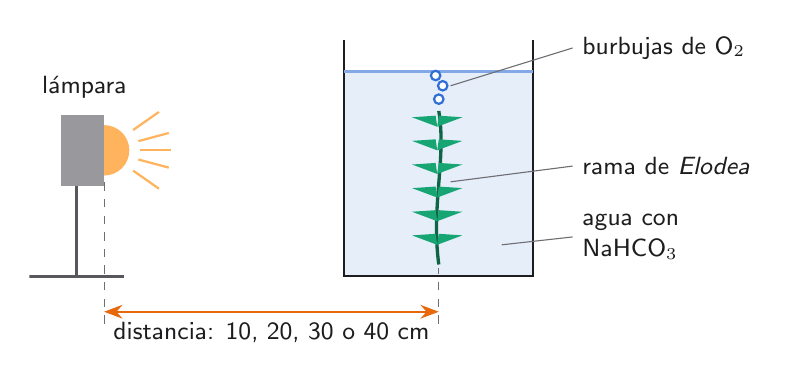
\begin{tikzpicture}[font=\small]
% lampara
\fill[narc] (0.55,1.6) circle (0.32);
\fill[gris!70] (0,1.15) -- (0.55,1.15) -- (0.55,2.05) -- (0,2.05) -- cycle;
\draw[gris!80!black,very thick] (0.2,1.15) -- (0.2,0) -- (-0.4,0) -- (0.8,0);
\foreach \a in {-35,-15,0,15,35} \draw[narc,thick] ($(0.55,1.6)+(\a:0.45)$) -- ($(0.55,1.6)+(\a:0.85)$);
\node[text=tinta] at (0.3,2.4) {lámpara};
% vaso
\fill[azul!12] (3.6,0) rectangle (6.0,2.6);
\draw[tinta,thick] (3.6,3.0) -- (3.6,0) -- (6.0,0) -- (6.0,3.0);
\draw[azul!60,thick] (3.6,2.6) -- (6.0,2.6);
% elodea
\draw[menta!60!black,very thick] (4.8,0.15) .. controls (4.7,0.9) and (4.9,1.5) .. (4.8,2.1);
\foreach \y in {0.4,0.7,1.0,1.3,1.6,1.9} {
  \fill[menta] (4.78,\y) -- ++(0.32,0.12) -- ++(-0.30,0.02) -- cycle;
  \fill[menta] (4.78,\y) -- ++(-0.32,0.12) -- ++(0.30,0.02) -- cycle;}
\foreach \p in {(4.8,2.25),(4.85,2.42),(4.76,2.55)} \draw[azul,thick,fill=white] \p circle (0.06);
% rotulos
\draw[gris] (4.95,2.42) -- (6.5,2.9) node[right,text=tinta] {burbujas de O$_2$};
\draw[gris] (4.95,1.2) -- (6.5,1.4) node[right,text=tinta] {rama de \textit{Elodea}};
\draw[gris] (5.6,0.4) -- (6.5,0.5) node[right,text=tinta,align=left] {agua con\\NaHCO$_3$};
% distancia
\draw[{Stealth}-{Stealth},nar,thick] (0.55,-0.45) -- node[below,text=tinta] {distancia: 10, 20, 30 o 40 cm} (4.8,-0.45);
\draw[gris,dashed] (0.55,-0.6) -- (0.55,1.2);
\draw[gris,dashed] (4.8,-0.6) -- (4.8,0.1);
\end{tikzpicture}
\end{document}
